% !TeX spellcheck = en_US
% !TeX root = ../build/road-to-scalability.tex
% !TeX TXS-program:compile = txs:///xelatex/[--shell-escape]


%%%%%%%%%%%%%%%%%%%%%%%%%%%%%%%%%%%%%%%%%%%%%%%%%%%%%%%%%%%%%%%%%%%%%%%%%%
\section{Blockchain Scalability}



%%%%%%%%%%%%%%%%%%%%%%%%%%%%%%%%%%%%%%%%%%%%%%%%%%%%%%%%%%%%%%%%%%%%%%%%%%
\subsection{Introduction}

A \textbf{blockchain} is a decentralized and peer-to-peer network that employs cryptographic techniques to securely host applications, store data, and facilitate the seamless exchange of digital assets that represent real-world currency. Figure \ref{fig:blockchain} illustrates a blockchain, wherein blocks are linked via the hash of the preceding block.

\begin{figure}[H]
\centering
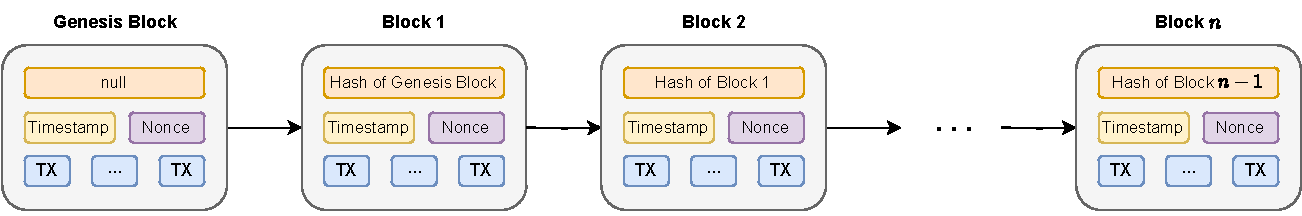
\includegraphics[width=\columnwidth]{\zkevmdir/figures/concepts/road-to-scalability/blockchain-schema.drawio}
\caption{Visual representation of a Blockchain.}
\label{fig:blockchain}
\end{figure}

The issue of \textbf{blockchain scalability} emerges as a foundational challenge within the realm of decentralized blockchain networks, and it undoubtedly stands as the most significant bottleneck in their development. This problem is related with the capacity and efficiency of these networks as they grow in terms of transaction volume. More specifically, as more transactions are sent to a blockchain network, its ability to process and validate these transactions in a timely and cost-effective manner becomes increasingly restricted.

The term \textit{scalability trilemma} was first coined by Vitalik Buterin to describe the inherent tension between three properties that a high-performing blockchain platform must have: \textbf{decentralization}, \textbf{security} and \textbf{scalability}.

\begin{enumerate}

\item \textbf{Decentralization:} This denotes the blockchain's capacity to operate without relying on trust relationships with a limited group of highly centralized entities.

\item \textbf{Security:} This represents the blockchain's capability to withstand attacks from a substantial proportion of participating nodes, ideally around 50\%.

\item \textbf{Scalability:} This refers to the blockchain's ability to augment the amount of processed transactions per second (TPS), increasing the overall system throughput.

\end{enumerate}

The \textit{trilemma} refers to the belief that blockchain platforms can only achieve two of these three goals effectively. Blockchain scalability is a critical concern because it impacts the network's ability to maintain decentralization, security, and usability while accommodating a growing user base and transaction load. Addressing this problem is essential for realizing the full potential of blockchain technology.

\subsection{Blockchain Scalability Strategies}

An EVM-based blockchain is a blockchain that utilizes the Ethereum Virtual Machine as its underlying computational engine. Intuitively speaking, we can conceptualize an EVM-based layer 1 blockchain as a set of states, each of them encapsulating the account balances, nonces, bytecode for smart contracts, storage values, and more. After \textbf{executing} a block of transactions at state $S_i$ using the EVM runtime environment, a new state $S_{i+1}$ appears, as shown in Figure \ref{fig:state-sequence}. The  \textbf{Ethereum World State}, as we saw in the previous section, is represented by the root of a Merkle Tree containing data for each of the Ethereum accounts. This state creation iterative process serves as the foundation for constructing a blockchain.

\begin{figure}[H]
\centering
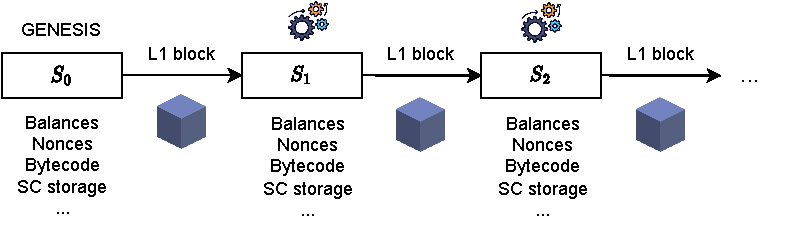
\includegraphics[width=0.95\columnwidth]{\zkevmdir/figures/concepts/road-to-scalability/ethereum-layer1.drawio}
\caption{Blockchain portrayed as a Sequence of States. }
\label{fig:state-sequence}
\end{figure}

In this scenario, transactions are both \textbf{available} to the entire network, ensuring visibility for all users, and are \textbf{executed} by the EVM runtime environment of each node.

\paragraph*{More transactions per block}

The initial strategy we can employ to enhance blockchain scalability involves increasing the number of transactions per block. This approach carries inherent risks that demand careful consideration. More specifically, as the volume of transactions per block surges, a significant number of blockchain nodes may find themselves stretched to their resource limits. Consequently, this escalation in resource demand can potentially lead to centralization, where the network becomes dominated by powerful nodes.

\paragraph*{Sharding}

Another strategy for scaling consists in the division of the network's workload into discrete segments, known as shards. In this approach, each node within the blockchain network is assigned responsibility for managing a specific shard. Consequently, a node only handles transactions of a particular shard. The sharding strategy involves using the existing L1 blockchain as a consolidation chain, which will be subsequently designated as the L1 \textbf{beacon chain}. The beacon chain serves as a central coordinating entity. Within the sharding strategy, there exist several approaches:

\begin{enumerate}[(a)]

\item In this approach, individual shards, which themselves function as distinct chains within the network, are tasked with executing a subset of blocks. On one hand, each shard ensures availability, guaranteeing that transactions are accessible. This accessibility extends to all nodes operating within the shard, all of which require access to transaction data. On the other hand, each shard possesses the execution capability akin to that of the beacon chain.

In essence, as shown in Figure \ref{fig:sharding-chains}, this approach creates a scenario in which both data availability and transaction execution are inherent features of each individual shard.

\begin{figure}[H]
\centering
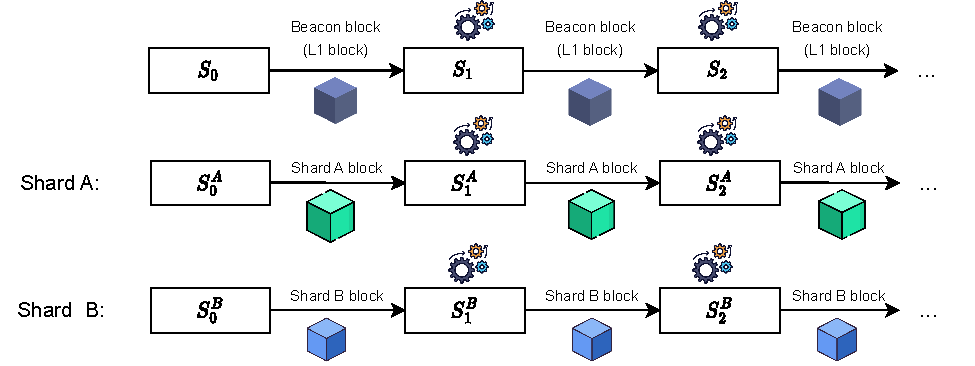
\includegraphics[width=.9\columnwidth]{\zkevmdir/figures/concepts/road-to-scalability/shard-chains.drawio}
\caption{Diagram depicting the initial sharding strategy, where each shard possesses the capability to execute transactions.}
\label{fig:sharding-chains}
\end{figure}

Nonetheless, this approach gives rise to significant challenges for Ethereum specifications. Firstly, with this approach, Ethereum specifications must define the rules for managing the states of each individual shard. This entails the execution of transactions and how inter-shard communication should work. Henceforth, an inherent consequence of this approach is the potential hindrance to L1 ossification. In the context of Ethereum, ossification refers to the stabilization and immutability of the Layer 1 protocol. The need for L1 Ethereum to actively manage and adapt to the evolving requirements of each shard can impede the process of ossification, as it requires ongoing updates and adjustments to accommodate the dynamic nature of the network. In conclusion, this method generates a huge instability in the specificiations of the Ethereum layer (Layer 1).


\item In this approach, Ethereum specifications provide a single L1 execution layer providing execution, the beacon chain, maintaining a unified L1 execution layer responsible for transaction processing and ensuring the accessibility of data, together with a data availability sharding scheme (\href{https://eips.ethereum.org/EIPS/eip-4844}{EIP-4844: Shard Blob Transactions}). So, the shards are data shards, they can be defined as chains of data availability without the capacity of executing transactions. Only the beacon chain can execute transactions, as depicted in Figure \ref{fig:EIP4844}.

\begin{figure}[H]
\centering
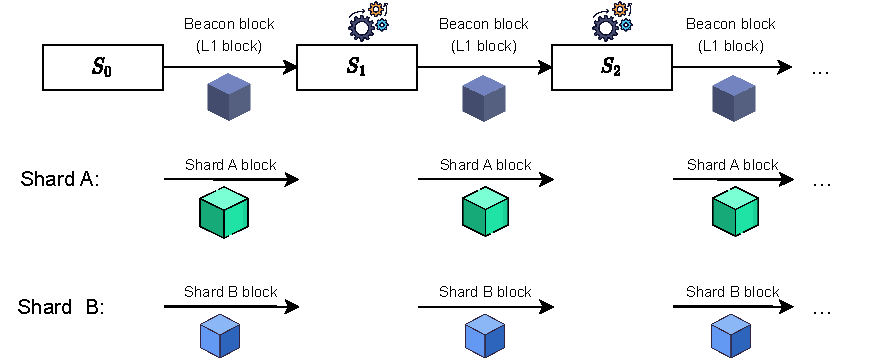
\includegraphics[width=.9\columnwidth]{\zkevmdir/figures/concepts/road-to-scalability/EIP-4844-concept.drawio}
\caption{Diagram illustrating the post EIP-4844 design. Transactions can only be executed on the beacon chain, as denoted by gears atop the states, while shards exclusively function as data shards.}
\label{fig:EIP4844}
\end{figure}

In this scheme, instead of conventional transactions, the blocks within each shard are now structured to contain \textbf{blobs} (binary large objects). These binary data hold no intrinsic meaning for the Layer 1; their intended purpose is to be decoded and processed by upper layers, which are widely known as \textbf{Layers 2}.


\end{enumerate}
